\section{External interface requirements}
  The system must be able to comunicate with a map service, in order to retrieve information about the users' position, send the best 
  route to the taxi drivers ,in case of shared ride, calculate the ETA for the passengers that requested a taxi.\\
  Also the application must be able to interact with a map service, due to allow passengers to select the meeting position.\\ 
\section { Functional Requirements}
For each goal, we define the specific function that we will have to implement;
\begin {itemize}
\item [G1]:
	\begin{itemize}
	\item Persons can create an account;
	\item Persons can log into their account;
	\item Passengers can select from a menu the option of requesting a taxi as soon as possible; 
	\item Passengers can insert their position filling an input form and confirm it;
	\item The system will receive the request and identify the zone in which the passenger is in;
	\item The system will forward the request to the first taxi in the selected zone queue and wait for an answer;
	\item If the taxist accepts, the system will remove him from the queue; otherwise it will append the taxist to the last position and
scan the list for a taxist to accept.
	\end{itemize}
\item [G2]:
	\begin{itemize}
	\item As soon as a taxist accepts a request, the system invokes the support system to calculate the ETA giving the position of the 
	taxi and the position of the passenger;
	\item The system will communicate the taxi code and the ETA.
	\end{itemize}
\item [G3]:
	\begin{itemize}
	\item Passengers can select from a menu the option of reserving a taxi for a chosen ride and date; 
	\item Passengers can insert the initial and final position, time and date, their email and confirm it;
	\item The system will receive the reservation and if it respects the 2 hour constraint it will send a confirmation;
	\item Ten minutes before the ride starts, the system allocates a taxi for it.
	\end{itemize}
\item [G4]:
	\begin{itemize}
	\item The application must have a selectable option labled:"share your ride", that allows passengers to enable the shared 
	ride service. In case of non reserved ride, the application will ask passengers the amount of time they can wait for others people;
	\item When the system receive a request of a shared ride, it will search for others shared ride requests starting from the same
	taxi zone, and going in the same direction;
	\item When a new passenger is added to a shared ride, the system will interact with the map service, in order to 
	retrieve a new route for the taxi driver, and to calculate new fees;
	\item When the timeout of one passengers ,added to the current ride, occur, the system will procede with the allocation of the taxi;
	\item After the taxi allocation, the passengers who requested the shared ride will receive, not only the taxi ID, but also 
	the fee they have to pay.
	\end{itemize}
\item[G5]:
	\begin{itemize}
	\item The system must forward a taxi request in the following cases:
	  \begin{itemize}
	   \item [1:] A passenger has requested a ride.
	   \item [2:] A taxi reservation is sheduled to begin in 10 minutes.
	  \end{itemize}
	\item If a taxi driver refuses to take care about a call, the system will move him at the end of the queue,and forward the
	request to the next taxi driver in the queue. If a queue is empty, the system will notify the passenger that there are no taxi available.
	\item If a taxe driver accepts to take care of the call, the system shall  remove him from the queue.
	\end{itemize}
\item [G6]:
	\begin{itemize}
	\item A taxi driver logged in into the system can select the button " Ready ", then the system will notify the system that 
	the logged user is ready to accept some passengr's call. The application also send the taxi driver's position detected with a GPS
	\item If the application needs to retrieve data from a GPS and this isn't available, it will remind  the user to turn it on.
	\item When the system receive a notification , by a taxi driver, informing that he is ready to take care of some passengers, 
	it will append the user in the queue corresponding to the taxi zone that include the position retrieved by the application.
	\end{itemize}
\item[G7]
	\begin{itemize}
	\item When a taxi driver is assigned to a shared ride, the system will send him the route he needs to follow, and the fee 
	amount every passenger have to pay
	\item When a driver is assigned to a non-shared ride, the system will send him the route he needs to follow, and the fee
	amount the passenger has to pay
	\end{itemize}
\item[G8]:
	\begin{itemize}
	\item  It is also neccessary to develop programmatic interfaces that allow to customize the system, adding new features.
	\end{itemize}
\end {itemize}
\begin{itemize}
 \item Passengers can access a section, in which they be able to check the ID of the taxi assigned to their ride 
 and manage ( delete or modify) an active reservation.
 \item When a passenger delete a reservation , the system will remove it from the reservation scheduler and, if a taxi 
 driver is already assigned, notify the taxist.
 \item A passenger can modify an active reservation changing position, date and time.
 \item The system will accept modification only if sent before the taxi allocation.
 \item The system will accept date and time modification if it occur at least two hours after the request or/and after the 
 previous reservation.
 \item A taxi driver have the possibility to remove himself from the queue by clicking the:``Disable'' button.
 \item The system will remove a taxi from the list if receive the corresponding request by the taxi driver, or if the taxist logged out.
 \item A master terminal interface must be implemented in order to allow, the stakeholder, to configure some parameters 
 (the number of the taxi zones, the set of positions belonging to each zone, the number of reports (per day, month and year)
  needed to automatically ban a user and the maximum number of reports ( per hour) a user can insert).
 \item Every time a report is added to a user, the system will check if the constraints inserted by the master terminal are satified,
 otherwise the system must automatically ban the user.
 \item The master terminal interface allows to manually ban users, or enable banned users.
 \item The system must refuse reports added by a user if the user has already reached the maximum number of reports ( per hour) decided
 by the master terminal.
 \item When the system refuse a report, a notification appear on the user screen, reminding him that he has already exceeded
 the maximum number of reports for that hour.
 \end{itemize}
 
\section{The World and the Machine}

Figure \ref{fig:world_and_machine} shows the model of the system, according to Jackson and Zave's model ``The world and the machine''

\begin{figure} [ht]
  \centering
  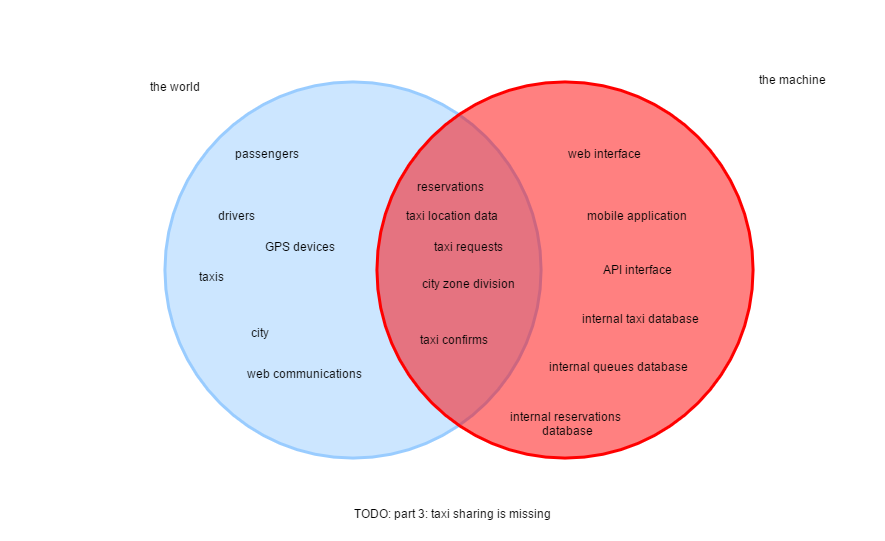
\includegraphics[scale=0.6]{../../notes/world and machine diagram.png}
  \caption{\label{fig:world_and_machine} the world and the machine}
\end{figure}

\section {Scenarios}
\begin{enumerate}
\item
Jon is driving back home while he notices a strange noise coming from his car. He decides to stop at the first garage
on the road and then call a taxi using an app he downloaded some weeks ago, MyTaxiService.
The mechanic checks the car and tells him that the problem is quite serious and the car must stay there for some maintenance. 
He opens MyTaxiService app and he accesses his account with his email and password. Then he inserts his position and selects "call a taxi".
The app informs him that he has to wait 5 minutes for taxi 13C to come over.
\item
Brandon is going to Moscow in three days and must be at the airport at 3:00 pm. Since the parking fee at the airport is very high
he decides to reserve a taxi that will lead him right near the airport entrance.
Brandon searches on his personal computer for a taxi service and finds MyTaxiService, creates an account inserting his email address and 
inventing a password,
he waits untill he receives a mail from MyTaxiService at the same email account he gave while signing in. He clicks the link in the mail
and now his account is valid. He can reserve a taxi from his house to the airport for that day and see the details in his "active taxi list".
\item
Eddard, a taxist, has just started a new day of work.
As soon as he gets in his vehicle he logs into his account, inserting his code and password.
Now he is connected with the system, a notification pop up informs him to turn on the gps. He activates the gps and he is sending correctly his position. 
Now he awaits for incoming calls.
\item
Robb, a taxist, receives a notification of an incoming call. The request comes from Mario Street, not far from his position.
Robb looks at the time, it's 12.58 meaning that his turn is over in two minutes, so he declines the request.
\item
Arya wants to go to an exibition downtown.
She has heard that the city centre will be closed at traffic but taxis will still be able to access. 
So she decides to book one, and in order to save some money she reserves a ride and enables the sharing option,
hoping that also others will use the taxi and join her.
She receives a notification from the taxi service in which they confirm the taxi and that 3 more people will use the same ride so the cost will be only of 5 dollars.
\item
Rickon, a taxist, receives a notification of an incoming call. It's a shared ride, the system provides him the route he has to follow, pick up a person in Golgi street then 
one in Grossich Street and leading them to Piazza Duomo, and the fees every passenger has to pay.
\end{enumerate}

\section {Use cases}
\begin{itemize}
\item Create an account
	\begin{center}
    	\begin{tabular}{ | l | p{11cm} |}
    	\hline
   	USE CASE & A user can create an account into myTaxiService \\ \hline
    	ACTORS & Visitor \\ \hline
     	Entry condition &  \\ \hline
     	Flow events & Visitor creates an account inserting his email address and choosing a password (longer than 8 characters). If he is willing to create an account as taxi driver, he must specify also his license number. The system processes the submission (in particular for a taxi driver checks the validity of the license given) and sends a confirmation mail to the given address in which there’s a link that the user must click to validate his account. \\ \hline
     	Exit condition & A new account is created \\ \hline
     	Exception &  If the email address is not correct or the user doesn’t confirm his account, the system will not consider any request from it. If the email address already belongs to an existing account or the password is shorter than 8 characters, the system gives an error before the user can continue.\\ \hline
    \end{tabular}
	\end{center}
	
\item Log in
	\begin{center}
   	 \begin{tabular}{ | l | p{11cm} |}
   	 \hline
   	USE CASE & A user can access his account\\ \hline
   	 ACTORS & User\\ \hline
    	 Entry condition & User must have already created an account \\ \hline
    	 Flow events & User inserts his email and password.\\ \hline
  	   Exit condition & The user sees his homepage, the taxist interface if he is a taxi driver or a passenger interface if he is not.\\ \hline
  	   Exception &  If the email doesn't correspond to an account the system gives an error message;
            if email is correct but the password isn't, the system gives an error message;\\ \hline
    \end{tabular}
\end{center}

  \begin{figure} [h]
  \centering
  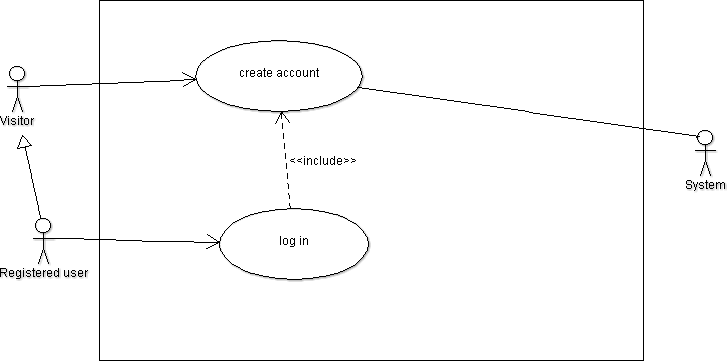
\includegraphics[scale=0.5]{register.png}
  \end{figure}

\newpage 

\item Request a taxi
	\begin{center}
   	 \begin{tabular}{ | l | p{11cm} |}
   	 \hline
   	USE CASE & A passenger can request a taxi\\ \hline
   	 ACTORS & Logged passenger \\ \hline
    	 Entry condition & Passenger must have already logged into his account \\ \hline
    	 Flow events & Passenger presses the button “call a taxi”, then inserts his adress (street/square, number). When he has done he clicks “send” button. The system checks if the location exists and then contacts the first taxist in the queue.
	When a taxist positively responds, the system look up for his position using his code and then calculates the ETA. Send both information, the taxi’s code and ETA to the user via a notification. \\ \hline
  	   Exit condition & A taxi, no more in the queue of available taxis, takes charge of the call and it’s moving towards the passenger.\\ \hline
  	   Exception &  If the location doesn’t exists or the system doesn’t find this address in the city map: the system sends an error 	message;
	If there are no taxis in the queue: the system sends a notification saying there are no available taxis;.\\ \hline
    \end{tabular}
	\end{center}

  \begin{figure} [h]
  \centering
  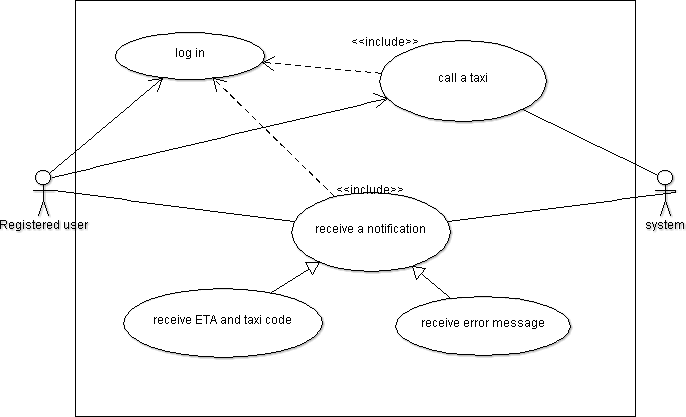
\includegraphics [scale=0.4]{callataxi.png}
  \end{figure}
	
\newpage
	
\item Book a taxi
	\begin{center}
   	 \begin{tabular}{ | l | p{11cm} |}
   	 \hline
   	USE CASE & A Passenger can book a taxi \\ \hline
   	 ACTORS & Logged passenger \\ \hline
    	 Entry condition & Passenger must have already logged into his account\\ \hline
    	 Flow events & Passenger presses the button “book a taxi”, then inserts the departure adress (street/square, number), 
    	 the destination address (street/square, number), the date (dd/mm/yyyy 00.00). He can select the shared ride option. 
    	 When he has filled all fields, he clicks “send” button. The system checks if the location exists and if the date respects 
    	 the constraints then sends a confirmation back to the user and saves the reservation in the scheduler system for the day it 
    	 occurs and in the queue where the ride will start.\\ \hline
  	   Exit condition & A taxi is allocated ten minutes before the ride begins, and the passenger can see in his active taxi list the reservation.\\ \hline
  	   Exception &  If the location doesn’t exists or the system doesn’’t find this address in the city map: the system sends an error message;
If the date doesn’t respect the constraints an error message is sent.\\ \hline
    \end{tabular}
\end{center}
\item Book a shared taxi ride
	\begin{center}
   	 \begin{tabular}{ | l | p{11cm} |}
   	 \hline
   	USE CASE & A Passenger can book a taxi with shared ride option\\ \hline
   	 ACTORS & Logged passenger \\ \hline
    	 Entry condition & Passenger must have already logged into his account \\ \hline
    	 Flow events & Passenger performs the same operation as booking a traditional 
    	 ride but selects also the share ride option. Now the input form will also ask him
    	 which destinations he wants to share. When he has done he clicks “send” button. 
    	 The system checks if the location exists and if the date respects the constraints 
    	 then sends a confirmation back to the user and saves the reservation for the day 
    	 it occurs and in the queue where the ride will start, in addition it will search 
    	 for other reservations with shared option enabled that could have parts of the way 
    	 in common and arrange a special route the taxist will follow.\\ \hline
  	   Exit condition & A taxi is allocated ten minutes before the ride begins, and the 
  	   passenger can see in his active taxi list the reservation.
The system will send a notification with the price the user must pay.\\ \hline
  	   Exception &  If the location doesn’t exists or the system doesn’t find this address in the city map: the system sends an error message;
If the date doesn’t respect the constraints an error message is sent\\ \hline
    \end{tabular}
	\end{center}
\item Modify a booked ride
	\begin{center}
   	 \begin{tabular}{ | l | p{11cm} |}
   	 \hline
   	USE CASE & A Passenger can modify a previous reservation\\ \hline
   	 ACTORS & Logged passenger \\ \hline
    	 Entry condition & Passenger must have already logged into his account and booked a ride, shared or not\\ \hline
    	 Flow events & Passenger enters his taxi calls and visualizes all the active rides he booked. He can modify all the parameters (start, destination, date).
In addition he can also delete a reservation.\\ \hline
  	   Exit condition & The modification/deletion is effective.\\ \hline
  	   Exception &  If the location doesn’t exists or the system doesn’t find this address in the city map: the system sends an error message;
If the date doesn’t respect the constraints an error message is sent\\ \hline
    \end{tabular}
	\end{center}
	
  \begin{figure} [h]
  \centering
  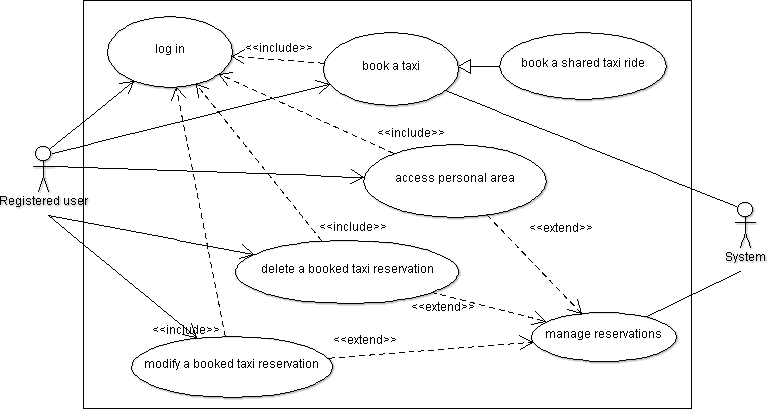
\includegraphics [scale=0.5]{bookataxi.png}
  \end{figure}
	
\newpage

\item Answer a call
	\begin{center}
   	 \begin{tabular}{ | l | p{11cm} |}
   	 \hline
   	USE CASE & A taxist can answer a call\\ \hline
   	 ACTORS & Logged taxist \\ \hline
    	 Entry condition & Taxist must be working and available, the system must forward a valid request \\ \hline
    	 Flow events & Taxist receives a notification on his mobile, with information about the ride ( route to follow, time).
He displays two option, accept or refuse. If he accepts he takes charge of the call otherwise he waits for another call. In the first case his code is sent to the system.\\ \hline
  	   Exit condition & If the taxist accepts, he is no more visible in that queue to the system.
If he refuses, he will be moved from first position in the queue to the last one.\\ \hline
  	   Exception &  \\ \hline
    \end{tabular}
\end{center}
\item Set availability
	\begin{center}
   	 \begin{tabular}{ | l | p{11cm} |}
   	 \hline
   	USE CASE & A taxist can render himself availablel\\ \hline
   	 ACTORS & Logged taxist \\ \hline
    	 Entry condition & Taxist must be working \\ \hline
    	 Flow events & Taxist sends his availability to the system pushing the “ready” button.\\ \hline
  	   Exit condition & The system receives his position and puts him in the queue in which he is in.\\ \hline
  	   Exception &  If the taxist hasn’t abilitate the gps, the app notifies him to turn it on.\\ \hline
    \end{tabular}
\end{center}

  \begin{figure} [h]
  \centering
  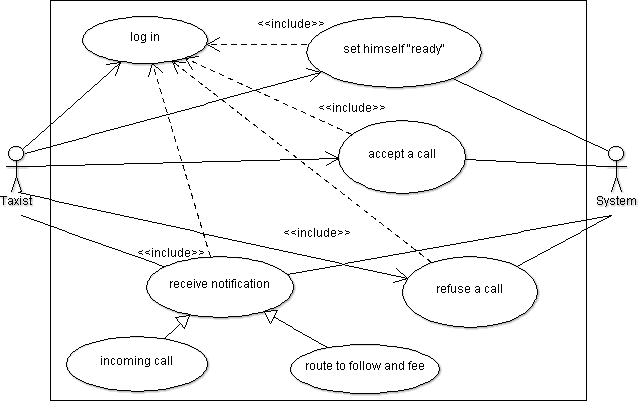
\includegraphics [scale=0.5]{taxist.png}
  \end{figure}

\end{itemize}

\newpage

\subsection{Sequence diagrams}
  \begin{figure} [h]
  \centering
  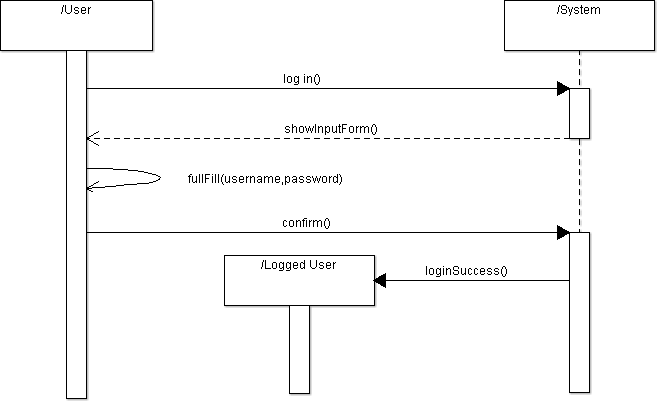
\includegraphics [scale=0.5]{sequencelogin.png}
  \end{figure}
\newpage

  \begin{figure} [h]
  \centering
  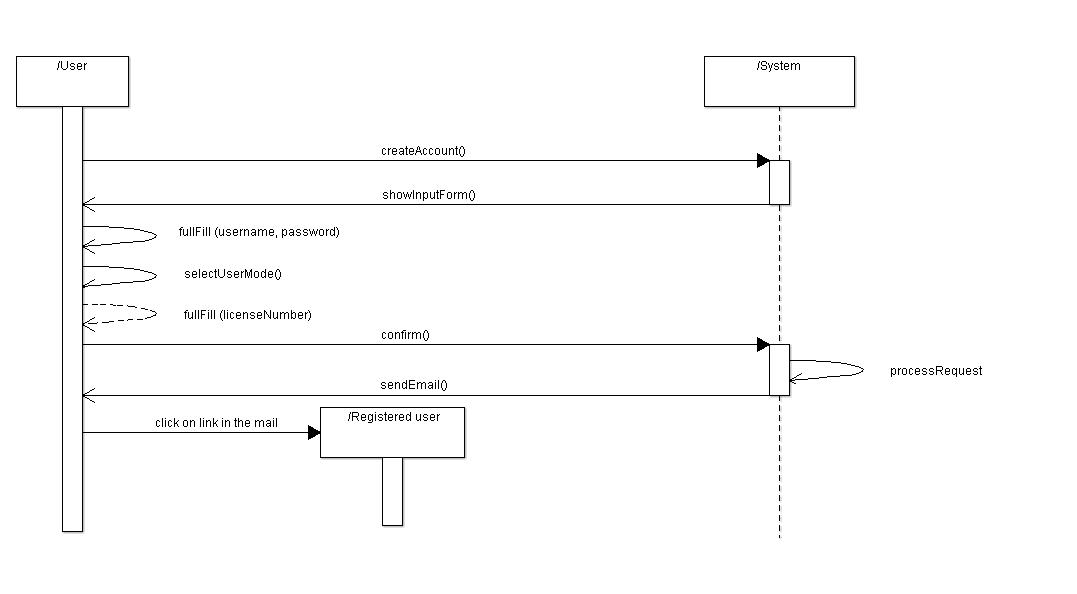
\includegraphics [scale=0.4]{sequenceregister.png}
  \end{figure}
\newpage

  \begin{figure} [h]
  \centering
  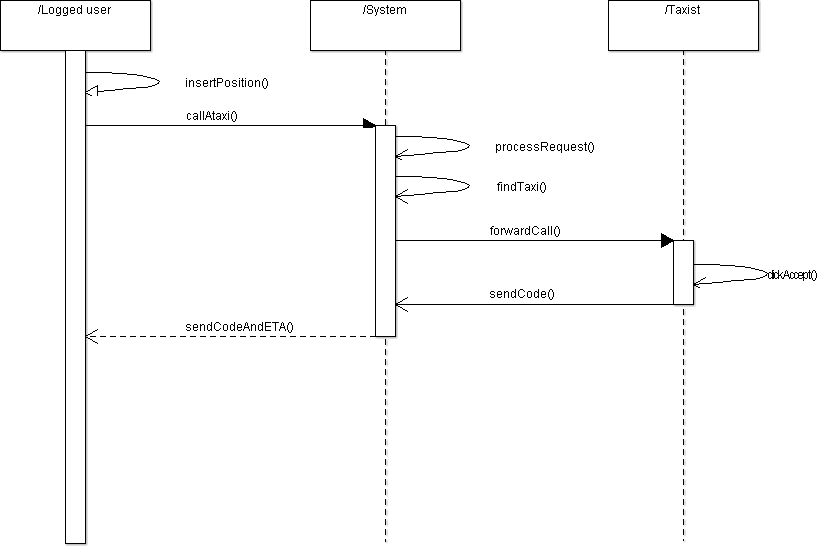
\includegraphics [scale=0.4]{sequencecall.png}
  \end{figure}
\newpage

  \begin{figure} [h]
  \centering
  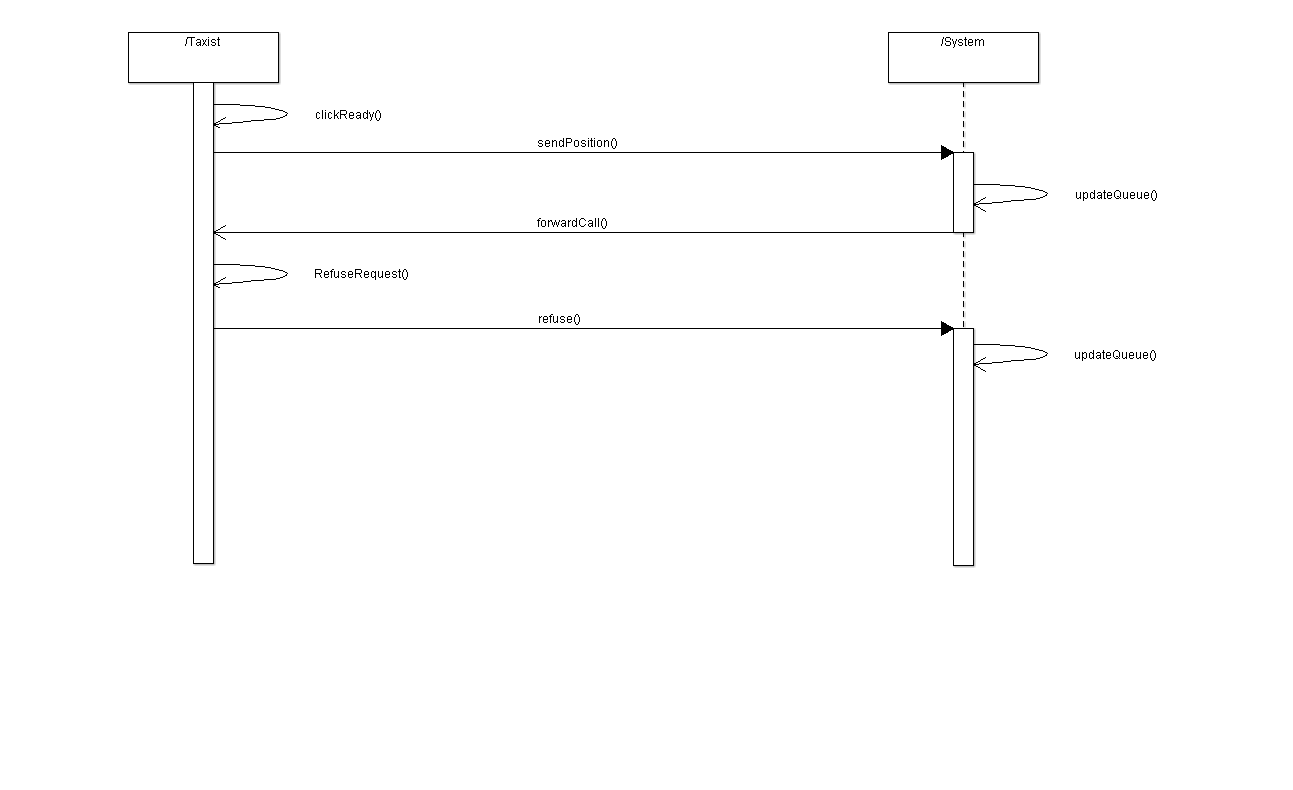
\includegraphics [scale=0.4]{sequencerefuse.png}
  \end{figure}
\newpage

\section{Software system attribute}
  \subsection{Reliability}
  In order to easily react against failure, the system will make a backup of all the server and save it on a cloud service.
  \subsection{Availability}
  The system is completely automatized, so it will be available every day at every time, except for the first Wednesday 
  of every month from ~20:00 to ~23:00 , when the server will be disconnected for maintenance, update and backup.
  \subsection{Security}
  The servers will be protected from external attack by adding two firewalls, located: between the network and the application server, 
  and between the application server and a the data server.
  Furthermore, all communications between user and server will be protected via Transport Layer Security.
  \subsection{Maintainability}
  The application must provide set of API for the purpose of adding new features in future time.
  Those API must be thoroughly documented; the core system must be documented as well.
  \subsection{Portability}
  The server side application could be deployed on any platform supporting JRE-7.\\
  The mobile application shall be developed for the major mobile operating systems ( Android , iOS, Windows phone).
  The web application shall be compatible with the most widely used browsers ( Mozilla Firefox, Google Chrome, Safari, Internet Explorer, Microsoft Edge) % >.<                                                                                                                                                                                                                                                                                                                                                                                                                                                                                                                                                                                                                                                                                                                                                                                                                                                                                                                                                                                                                                                                                                            
